\documentclass{article}

\usepackage[english]{babel}
\usepackage[utf8]{inputenc}
\usepackage[T1]{fontenc}
\usepackage{amsmath, amsfonts, amssymb, amsthm}
\usepackage{tikz}
\usepackage{csquotes}
\usepackage{stmaryrd}


\usepackage[backend=biber,citetracker=true]{biblatex}
\addbibresource{bibli.bib}
\usepackage{color}
\usepackage{subcaption}
\usepackage{graphicx}
\usepackage{./tex/sty/scribe}
\usepackage{float}

\newcommand*{\AIC}{\mathrm{AIC}}
\newcommand*{\BIC}{\mathrm{BIC}}

%\usepackage{epsfig}
%\usepackage{ulem, stmaryrd, dsfont}


\author{Fanchon Herman}


\begin{document}
\begin{titlepage} 
	\newcommand{\HRule}{\rule{\linewidth}{0.5mm}}
	
	\center
	
	\textsc{\LARGE University of Montpellier}\\[1.5cm]
	
	\textsc{\Large Master 2 Biostatistique }\\[0.5cm] 
	
	\textsc{\large HMMA$307$ Project}\\[0.5cm] 

	\HRule\\[0.4cm]
	
	{\huge\bfseries Linear Mixed Models}\\[0.4cm] 
	
	\HRule\\[1.5cm]
	
	\begin{minipage}{0.4\textwidth}
		\begin{flushleft}
			\large
			\textit{Student: }\\
			Fanchon Herman
		\end{flushleft}
	\end{minipage}
	~
	\begin{minipage}{0.4\textwidth}
		\begin{flushright}
			\large
			\textit{Teacher: }\\
			Joseph Salmon\\
		\end{flushright}
	\end{minipage}
		\vfill 
	
	{\large 2020-2021} 

		\vfill\vfill
		
\centering

\includegraphics[width=0.2\textwidth]{./images/Logo}


	
	 
	%----------------------------------------------------------------------------------------
	
	\vfill 
\end{titlepage}

\tableofcontents
\newpage
%%%%%%%%%%%%%%%%%%%%%%%%%%%%%%%%%%%%%%%%%%%%%%%%%%%%%%%%%%%%%%%%%%%%%%%%%%%%%%%
%%%%%%%%%%%%%%%%%%%%%%%%%%%%%%%%%%%%%%%%%%%%%%%%%%%%%%%%%%%%%%%%%%%%%%%%%%%%%%%
\section*{Introduction}

Linear mixed models are an extension of simple linear models to allow fixed and random effects. A fixed effect is a parameter that remains constant and random effects are parameters that are random variables. These types of models are widely used when the data is not independent.

In this project, we use the dataset from Grodner and Gibson, Expt $1$.
This dataset deals with subject and object relative clause data from English.
Grodner and Gibson analyzed the reading times at the relative clause verb in a self-paced reading study. In this dataset, we have $672$ observations and $42$ subjects.

Throughout this project, we are interested in three main types of linear mixed models. For each model, we explain the statistical model and the model outputs from $\texttt{Python}$. In addition, we take care to validate the models and select the most judicious one using various criteria.
%%%%%%%%%%%%%%%%%%%%%%%%%%%%%%%%%%%%%%%%%%%%%%%%%%%%%%%%%%%%%%%%%%%%%%%%%%%%%%%
%%%%%%%%%%%%%%%%%%%%%%%%%%%%%%%%%%%%%%%%%%%%%%%%%%%%%%%%%%%%%%%%%%%%%%%%%%%%%%%


%%%%%%%%%%%%%%%%%%%%%%%%%%%%%%%%%%%%%%%%%%%%%%%%%%%%%%%%%%%%%%%%%%%%%%%%%%%%%%%
%%%%%%%%%%%%%%%%%%%%%%%%%%%%%%%%%%%%%%%%%%%%%%%%%%%%%%%%%%%%%%%%%%%%%%%%%%%%%%%
\section{Model type 1 - Varying intercepts}
We first start to analyze a mixed linear model by varying the intercept.
We model individual means with random intercepts.
The previous statement adjusts the grand mean estimates of the intercept by a term for each subject. Only the mean and standard deviation of the intercept distribution are estimated instead of $42$ intercepts for each subject.
This saves degrees of freedom because less parameter estimation is required.
We  model these individual differences by assuming different random intercepts for each subject. So, each subject is assigned a different intercept value.

\subsection{Equation of the model}
The mathematical equation of the model is:
\begin{equation}
y_{ij}= \beta_0 + u_{0i} + \beta_1 \times so_{ij} + \varepsilon_{ij}\enspace. \label{rel:mod1}
\end{equation}
In this model, $i$ indexes subjects and $j$ indexes items. So, $i \in \llbracket1,42\rrbracket$ and $j \in \llbracket1,16\rrbracket.$
Besides, the intercept $\beta_0$ and slope $so_{ij}$  represent two fixed effects and $u_{0i}$ represents a random effect. The model has a different intercept $\beta_0 + u_{i0}$ for each subject $i$. In addition, $\beta_1$ corresponds to the slope parameter.

In the model \eqref{rel:mod1}, we have two sources of variance which are:
\begin{itemize}
    \item $u_{0i} \sim \mathcal{N}(0,\sigma_{u0}) \text{ , } \sigma_{u0}>0$, iid on $i$ \enspace,
    \item $\varepsilon \sim \mathcal{N}(0, \sigma) \text{ , } \sigma >0$, iid on $i$ and $j$\enspace,
    \item $\forall i \text{,} j \text{ , } u_{i0} \perp \!\!\! \perp \varepsilon_{ij}$\enspace.
\end{itemize}

In addition, these two standard deviations determine the standard error of the $\beta_1$ slope parameter.

From the model \eqref{rel:mod1}, we can calculate its expectation and variance: 
$$\E(y_{ij})=\beta_0 + \beta_1 \E(so_{ij}) \enspace,$$
$$\Var(y_{ij})=\sigma_{u0} + \beta_1^2 Var(so_{ij}) + \sigma \enspace.$$

\subsection{Model explanations}
The output of the model is:
\begin{center}
    \begin{tabular}{|c|c|c|c|c|c|}
    \hline
         & Coef & Std.Err & z & P>|z| &$\text{IC}(95\%)(\text{Coef})$  \\
         \hline \hline
        Intercept & 5.883 & 0.051 & 115.502 & $\simeq$0.000 & 5.783 5.983\\
         so & 0.062 & 0.015 & 4.205 & $\simeq$0.000 & 0.033 0.091 \\
         Group var &  0.100 & 0.065 &  & &  \\
         \hline
    \end{tabular}
    \captionof{table}{Numerical outputs of the mixed linear model carried out from \texttt{Python}.} 
\end{center}


By the results of the mixed linear model, we have:
$\hat{\sigma}_{u0}=0.316$ and $\hat{\sigma}=0.382$.

The theoretical formulas of the estimators are:
\begin{itemize}
    \item $\hat{\sigma}=\dfrac{1}{n-J} \sum_{j=1}^{J} \sum_{i=1}^{n_j} (y_{ij}-\Bar{y}_{:j})^2$,
    \item $\hat{\sigma}_{u0}=\dfrac{\dfrac{1}{J-1} \sum_{j=1}^J n_j(\Bar{y}_{:j}-y_n)^2 - \hat{\sigma}}{n^2 - \sum_{j=1}^J n_j^2}$,
\end{itemize}
where $n_j$ corresponds to the number of repetitions of the phenomenon, $n=\sum_{j=1}^J n_j$ and $\Bar{y}_{:j}=(n_j)^{-1}\sum_{i=1}^{n_j} y_{ij}$.

In addition, we can see that the intercept (subject) explains around $40\%$ of the variations. Indeed, we have: $$\dfrac{\hat{\sigma}_{u0}^2}{\hat{\sigma}_{u0}^2+\hat{\sigma}^2} \simeq \dfrac{0.0999}{0.0999+0.146} \simeq 0.4.$$
So, after the variance explained by fixed effects, the differences between the subjects explain about $40\%$ of the remaining variance.

We can also see that the confidence interval 
threshold $\alpha=5\%$ of the variable so is $[0.033, 0.091]$. This interval does not include the value $0$, so we can say that the feature \text{so} is significantly différent from $0$.
Now, let's visualize the adjustments to the grand mean for each subject.

\begin{figure}[H]
    \centering
    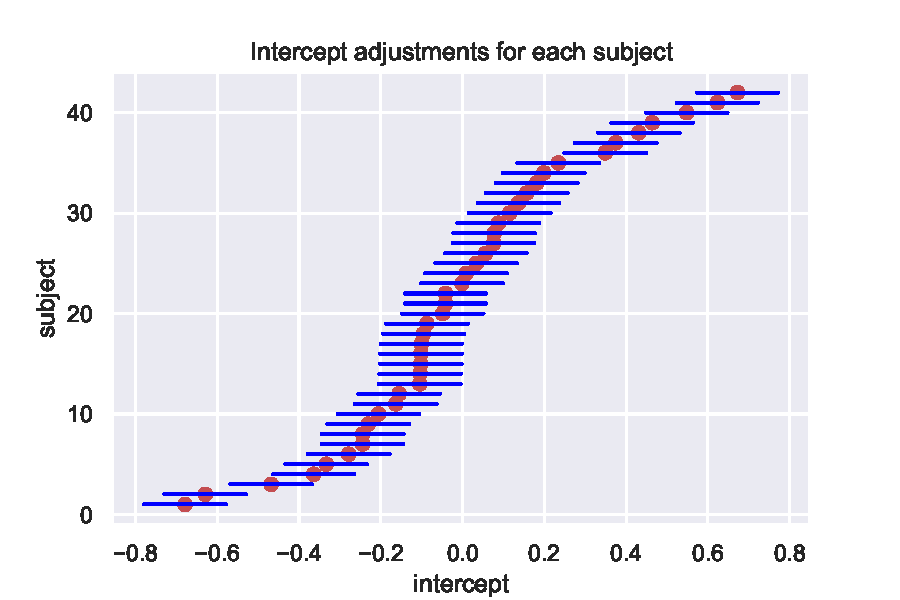
\includegraphics[scale=.65]{./images/model1_inter.pdf}
    \caption{Representation of the intercept adjustements by subject.}
    \label{fig:model1}
\end{figure}

In the Figure \ref{fig:model1}, we can note that our model produces a different intercept for each subject in addition to a parameter estimate for features logrt (log-transformed reading time) and $\text{so}$ (the contrast coding) which is constant between subjects. In addition, the error bars represent the $95\%$ confidence intervals. We can see that there is a large variability in the average reading times between subjects.

\subsection{Model validation}
Let's see how we can validate the model. In order to check the homogeneity, we plot the predicted values against the residuals. In addition, we also check the normality of the residuals.
\begin{figure}[H]
\centering
\begin{subfigure}{.5\textwidth}
  \centering
  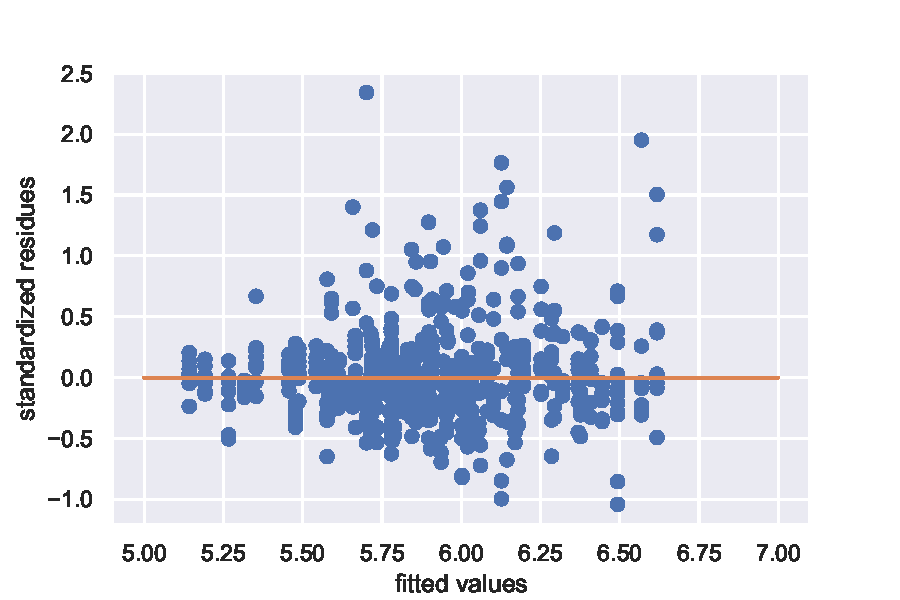
\includegraphics[width=1\linewidth]{./images/homo_mod1.pdf}
  \caption{Representation of the predicted by residual values.}
  \label{fig:homo_mod1}
\end{subfigure}%
\begin{subfigure}{.5\textwidth}
  \centering
  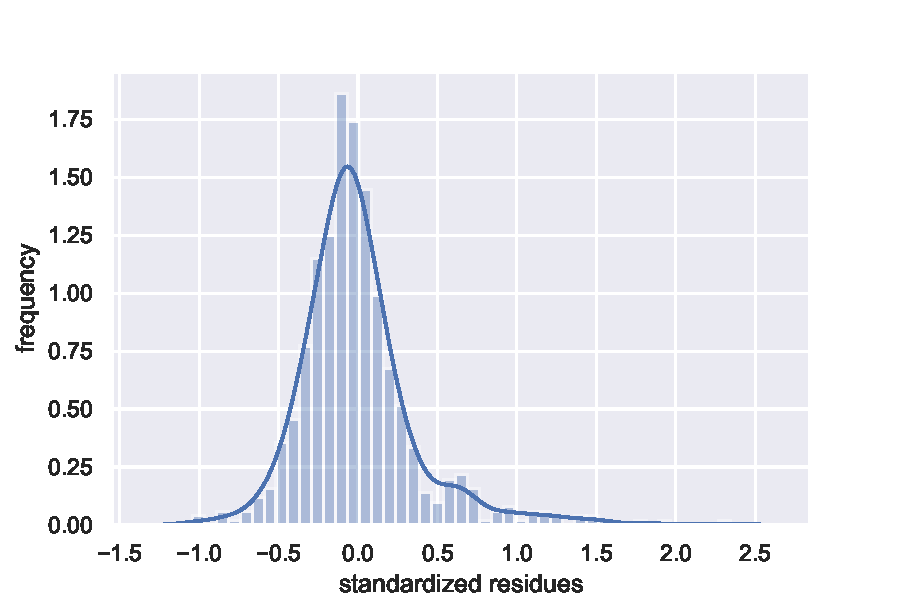
\includegraphics[width=1\linewidth, clip,trim={0cm 0cm 0cm 0.6cm} ]{./images/resid_norm.pdf}
  \caption{Representation of the normality of the residuals.}
  \label{fig:resid}
\end{subfigure}
\caption{Model validation of the first model.}
\label{fig:valid_1}
\end{figure}

In the Figure \ref{fig:valid_1}, we can note that the magnitude of the residuals suggests that the model seems to fit our data well. In addition, we can see that the normality of the residuals is verified.

\subsection{Model selection}
In order to evaluate the models, we can use the AIC criterion.
We calculate the AIC of the model \eqref{rel:mod1} to compare it with those of the other models defined hereafter. The AIC criterion is defined by:
\[ \AIC = 2k - 2\ln({\hat{L}}),\]
with  $k$ the number of estimated parameters in the model and $\hat{L}$ is the maximum likelihood of the model.


For practical reasons, we use the AIC formula defined using the deviance:
\begin{equation}
    \AIC=\text{deviance} + 2 \times (p+1)=(-2) \times \log(\text{likelihood}) + 2 \times (p+1).\label{AIC}
\end{equation}
In \eqref{AIC}, $1$ is for the estimated residual variance and $p$ is for all the other parameters.


Using the formula \eqref{AIC} and for our associated model, we find an AIC of approximately $735.6817$ (with a total of $4=3+1$ parameters).
We can also use the BIC criterion for model selection. The BIC criterion is defined by:
\begin{equation}
    \BIC= (-2) \times \log(\text{likelihood}) + (p+1) \times \log(n).\label{BIC}
\end{equation}
where $n$ the number of observations.
For our model, the BIC is approximately equal to $753.7227$.

%%%%%%%%%%%%%%%%%%%%%%%%%%%%%%%%%%%%%%%%%%%%%%%%%%%%%%%%%%%%%%%%%%%%%%%%%%%%%%%
%%%%%%%%%%%%%%%%%%%%%%%%%%%%%%%%%%%%%%%%%%%%%%%%%%%%%%%%%%%%%%%%%%%%%%%%%%%%%%%

%%%%%%%%%%%%%%%%%%%%%%%%%%%%%%%%%%%%%%%%%%%%%%%%%%%%%%%%%%%%%%%%%%%%%%%%%%%%%%%
%%%%%%%%%%%%%%%%%%%%%%%%%%%%%%%%%%%%%%%%%%%%%%%%%%%%%%%%%%%%%%%%%%%%%%%%%%%%%%%
\section{Model type 2 - Varying intercepts and slopes, without a correlation}

The first model suppose different intercepts by subjects. However, the slope remained the same for each subject. We will now study a second type of model by varying the intercepts and slopes, without correlation. 
As with the intercepts, only the mean and standard deviation of the slopes are estimated instead of $42$ separate slopes.

\subsection{Equation of the model}
The mathematical equation of the model is:
\begin{equation}\label{mod2}
    y_{ij}= \beta_0 + u_{0i} + (\beta_1 + u_{1i}) \times so_{ij} + \varepsilon_{ij} \enspace.
\end{equation}
In the model \eqref{mod2}, $i$ indexes subjects and $j$ indexes items. So, $i \in \llbracket1,42\rrbracket $ and $j \in \llbracket1,16\rrbracket$.

In the model \eqref{mod2}, we have three sources of variance which are:
\begin{itemize}
    \item $u_0 \sim \mathcal{N}(0,\sigma_{u0})$, $\sigma_{u0}>0$ \enspace,
    \item $u_1 \sim \mathcal{N}(0,\sigma_{u1})$, $\sigma_{u1}>0$\enspace,
    \item $\varepsilon \sim \mathcal{N}(0, \sigma)$, $\sigma>0$\enspace.
\end{itemize}

\subsection{Model explanations}
The output of the model is:
\begin{center}
    \begin{tabular}{|c|c|c|c|c|c|}
    \hline
         & Coef & Std.Err & z & P>|z| & $\text{IC}(95\%)(\text{Coef})$  \\
         \hline \hline
        Intercept & 5.883 & 0.051 & 115.496 & $\simeq$0.000 & 5.783 5.983\\
         so & 0.062 & 0.022 & 2.810 & $\simeq$0.005 & 0.019 0.105 \\
         Group var &  0.101 & 0.068 &  & & \\
         Group x so Cov & 0.020 & 0.022 & & &\\
         so Var & 0.012 & 0.013 & & &\\
         \hline
    \end{tabular}
    \captionof{table}{Numerical outputs of the mixed linear model carried out from \texttt{Python}.} 
\end{center}

First, by the results of the mixed linear model, we have:
$\hat{\sigma}_{u0}=0.317$, $\hat{\sigma}_{u1}=0.110$ and $\hat{\sigma}=\sqrt{0.1336}=0.366$.

Secondly, in order to determine if the slope is significantly different from $0$, we study its confidence interval.
Indeed, if its confidence interval at the $5\%$ threshold includes the value $0$, we can say that the slope is not significantly different from $0$.
The confidence interval of the slope is $[0.019, 0.105]$. So, this interval does not include $0$, we can affirm at the $5\%$ threshold that the slope is significantly different from $0$.
We can now visualize the adjustments to the intercept and slope for each subject.

\begin{figure}[H]
    \centering
    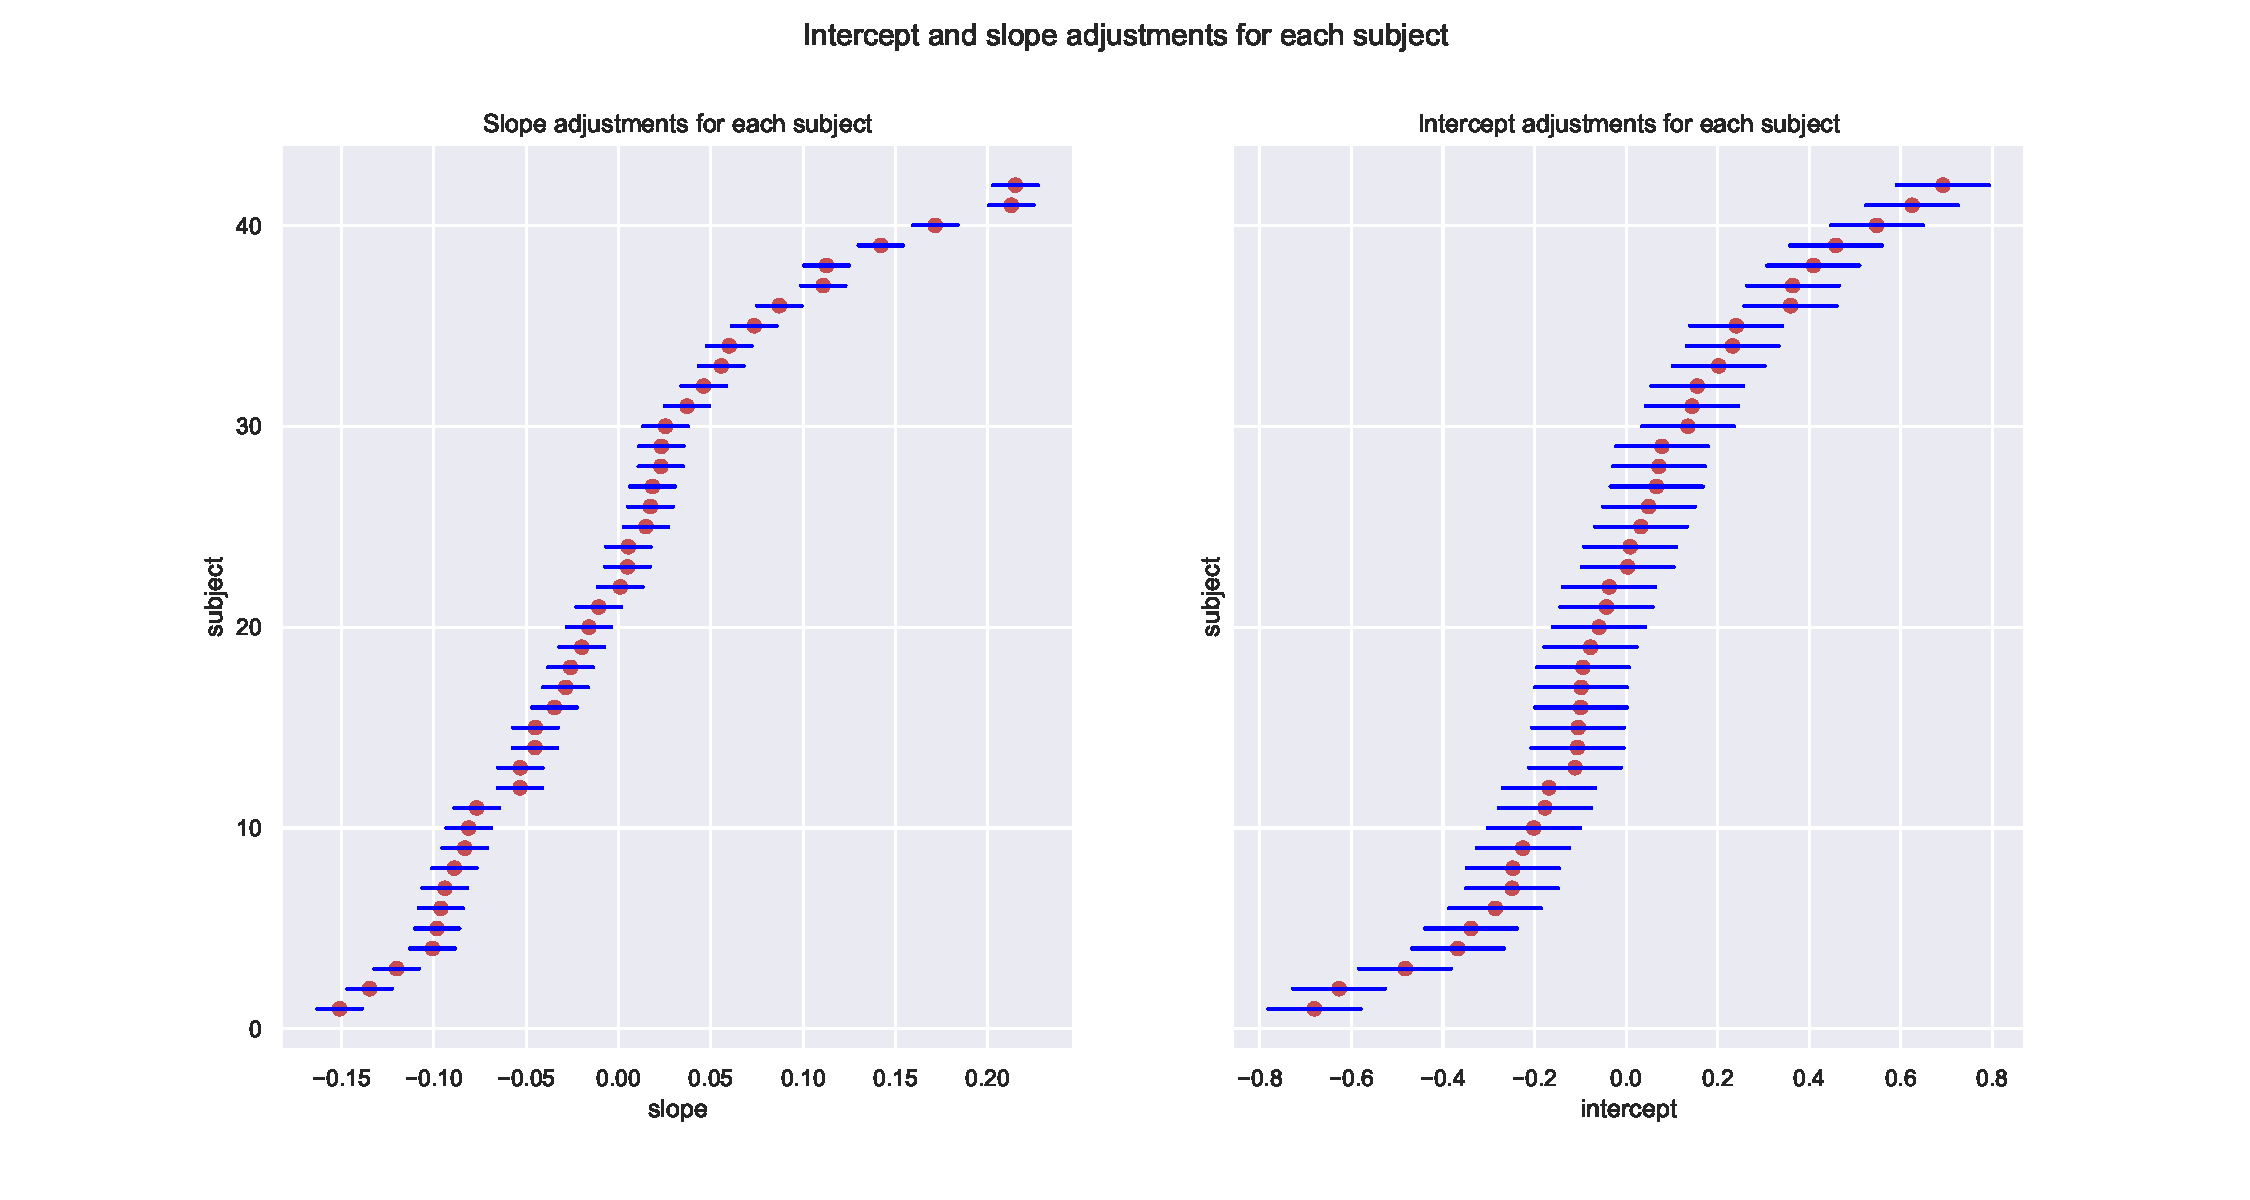
\includegraphics[scale=.42]{./images/model2_inter.pdf}
    \caption{Representation of the intercept and slope adjustements by subject.}
    \label{fig:model2}
\end{figure}

In the Figure \ref{fig:model2}, the error bars in the figure represent $95\%$ confidence intervals. We can note a little variation in slope between subjects. However, there is a large variability in the average reading times between subjects. We can note that our model produces a different intercept and slope for each subject.

\subsection{Model validation}
As before, we validate our model.
We plot the predicted values against the residuals to check the homogeneity. Moreover, we also check the normality of the residues.

\begin{figure}[H]
\centering
\begin{subfigure}{.5\textwidth}
  \centering
  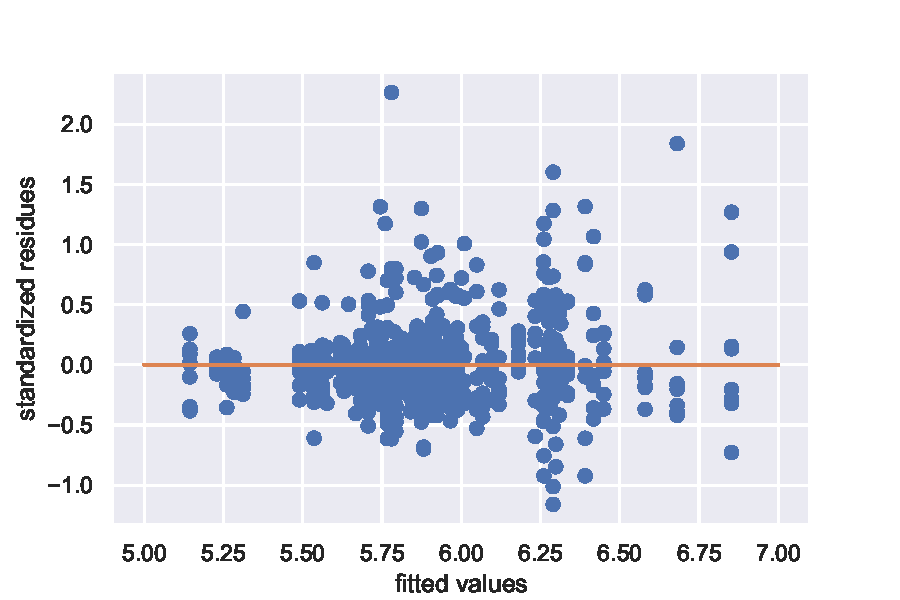
\includegraphics[width=1\linewidth]{./images/homo_mod2.pdf}
  \caption{Representation of the predicted by residual values.}
  \label{fig:homo_mod2}
\end{subfigure}%
\begin{subfigure}{.5\textwidth}
  \centering
  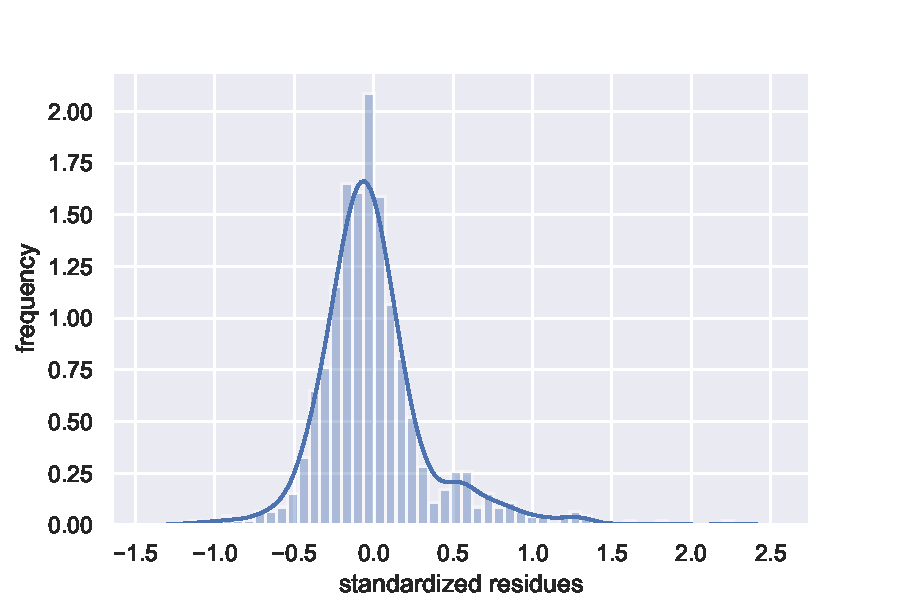
\includegraphics[width=1\linewidth, clip,trim={0cm 0cm 0cm 0.6cm} ]{./images/resid_norm_m2.pdf}
  \caption{Representation of the normality of the residuals.}
  \label{fig:resid_}
\end{subfigure}
\caption{Model validation for the second model.}
\label{fig:valid_2}
\end{figure}

In the Figure \ref{fig:valid_2}, we can note that the residuals seem to be not too far from the orange line. Meaning that the model fits our data well.
We also have the normality of the residuals.

\subsection{Model selection}
After studying two different models, we can compare these two models by looking at their AIC values.
Using the AIC formula defined from the deviance \eqref{AIC}, we obtain an AIC of approximately $709.1464$ (with a total of $5=4+1$ parameters). In addition, the value of the BIC criterion \eqref{BIC} is approximately equal to $731.5977$.
Since the previous model has a greater AIC and BIC values than this, we can say that this model is the less bad model for out of the two. Thus, this model has a greater predictive power than the previous model.

%%%%%%%%%%%%%%%%%%%%%%%%%%%%%%%%%%%%%%%%%%%%%%%%%%%%%%%%%%%%%%%%%%%%%%%%%%%%%%%
%%%%%%%%%%%%%%%%%%%%%%%%%%%%%%%%%%%%%%%%%%%%%%%%%%%%%%%%%%%%%%%%%%%%%%%%%%%%%%%


%%%%%%%%%%%%%%%%%%%%%%%%%%%%%%%%%%%%%%%%%%%%%%%%%%%%%%%%%%%%%%%%%%%%%%%%%%%%%%%
%%%%%%%%%%%%%%%%%%%%%%%%%%%%%%%%%%%%%%%%%%%%%%%%%%%%%%%%%%%%%%%%%%%%%%%%%%%%%%%
\section{Model type 3 - Varying intercepts and slopes, with correlation}
%%%%%%%%%%%%%%%%%%%%%%%%%%%%%%%%%%%%%%%%%%%%%%%%%%%%%%%%%%%%%%%%%%%%%%%%%%%%%%%
%%%%%%%%%%%%%%%%%%%%%%%%%%%%%%%%%%%%%%%%%%%%%%%%%%%%%%%%%%%%%%%%%%%%%%%%%%%%%%%

\subsection{Equation of the model}
The mathematical equation of the model is:
\begin{equation}
    y_{ij}= \alpha + u_{0i} + w_{0j}+(\beta + u_{1i} + w_{1j}) \times so_{ij} + \varepsilon_{ij}\enspace,\label{mod3}
\end{equation}
with 
\begin{itemize}
    \item $\varepsilon_{ij} \sim \mathcal{N}(0, \sigma)$, $\sigma>0$,
    \item
    $\begin{pmatrix}
    u_0 & u_1\\
    \end{pmatrix}^{\top}\sim \mathcal{N}\left(\begin{pmatrix}
    0 & 0\\
    \end{pmatrix}^{\top},\Sigma_u\right)$,
    \item 
    $\begin{pmatrix}
    w_0 & w_1\\
    \end{pmatrix}^{\top}\sim \mathcal{N}\left(\begin{pmatrix}
    0 & 0\\
    \end{pmatrix}^{\top},\Sigma_w\right)$.
\end{itemize}
where $\Sigma_u=\begin{pmatrix}
\sigma_{u0}^2  & \rho_u\sigma_{u0}\sigma_{u1}\\
\rho_u\sigma_{u0}\sigma_{u1} & \sigma_{u1}^2\\
\end{pmatrix} \text{ and } \Sigma_w=\begin{pmatrix}
\sigma_{w0}^2  & \rho_u\sigma_{w0}\sigma_{w1}\\
\rho_u\sigma_{w0}\sigma_{w1} & \sigma_{w1}^2\\
\end{pmatrix} $.

In this model \eqref{mod3}, we add item-level effects and also include correlation parameters.

\subsection{Model explanations}
The output of the model is:
\begin{center}
    \begin{tabular}{|c|c|c|c|c|c|}
    \hline
         & Coef & Std.Err & z & P>|z| & $\text{IC}(95\%)(\text{Coef})$ \\
         \hline \hline
        Intercept & 5.883 & 0.051 & 115.497 & $\simeq$0.000 & 5.783 5.983\\
         so & 0.062 & 0.022 & 2.810 & $\simeq$0.005 & 0.019 0.105 \\
         subject var &  0.101 &  &  & & \\
         subject x so Cov & 0.020 &  & & &\\
         so Var & 0.012 &  & & &\\
         item Var & 0.076 & & & &\\
         \hline
    \end{tabular}
    \captionof{table}{Numerical outputs of the mixed linear model carried out from \texttt{Python}.} 
\end{center}
The correlation between the varying intercepts and slopes for subjects is equal to $0.58$. They are moderately positively correlated.
In addition, the correlation between the varying intercepts and slopes for items is equal to $1$. We have a perfect positive correlation between us.
Let's visualize the adjustments to the intercept and slope for each subject.

\begin{figure}[H]
    \centering
    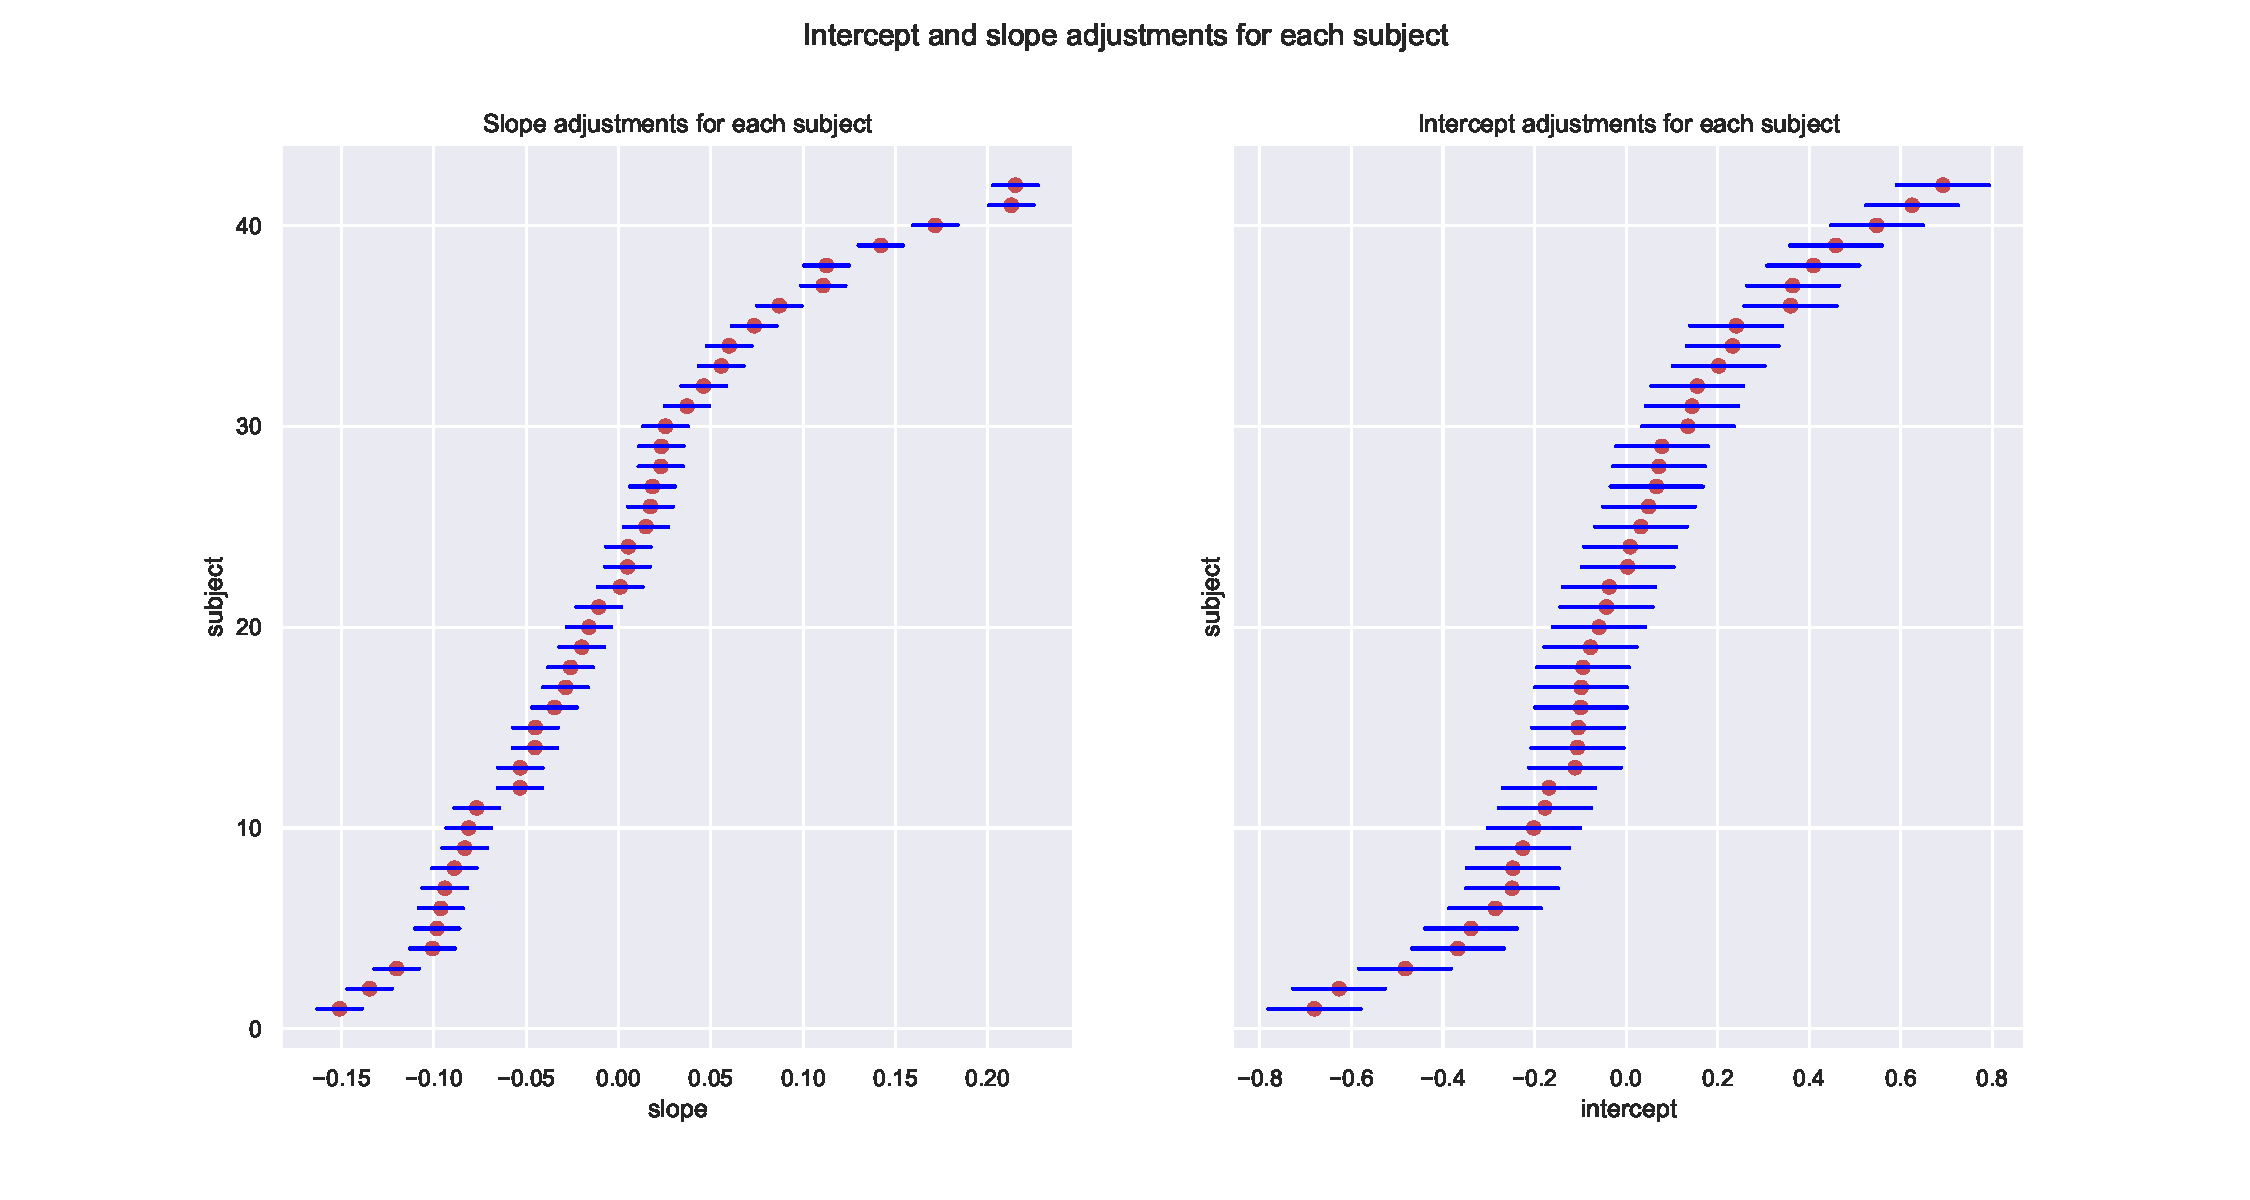
\includegraphics[scale=.42]{./images/model3_inter.pdf}
    \caption{Representation of the intercept and slope adjustements by subject.}
    \label{fig:model3}
\end{figure}

In the Figure \ref{fig:model3}, the error bars in the figure represent $95\%$ confidence intervals. We can note a little variation in slope between subjects and  a large variability in the average reading times between subjects. Like the previous model, we can note that our model produces a different intercept and slope for each subject. 

In order to visualize the correlation between intercept and slopes by subjects, we plot the slope adjustments against the intercept adjustments.
\begin{figure}[H]
    \centering
    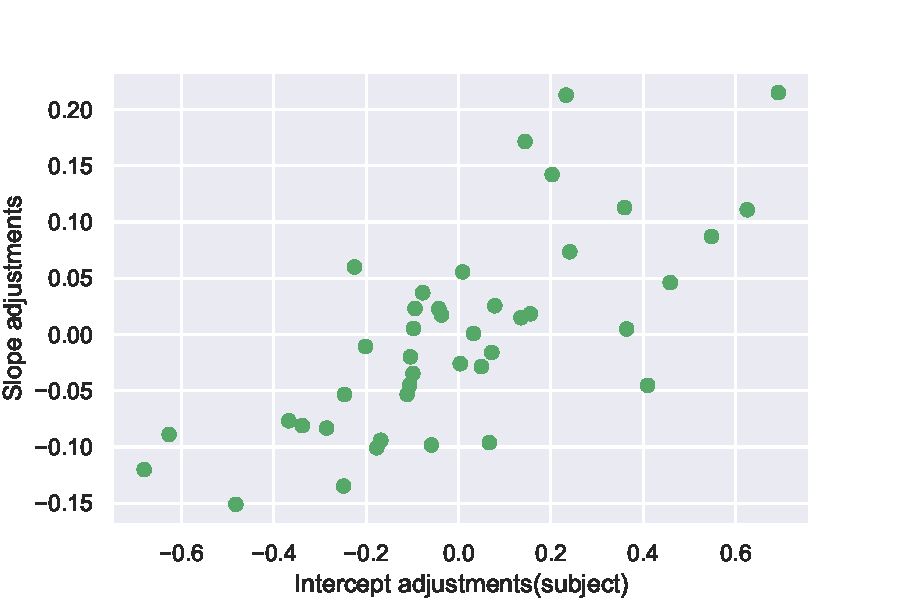
\includegraphics[scale=.65]{./images/adj_so_inter.pdf}
    \caption{Representation of the slope adjustments against the intercept adjustements.}
    \label{fig:adj_slope}
\end{figure}

On the Figure \ref{fig:adj_slope}, we recognize that the data could fit a linear model. Indeed, considering that there is some noise on the data, when the intercept gets higher, the slope adjustement also increases linearly. 

\subsection{Model validation}
Now, we validate this model \eqref{mod3}. To do this, we plot the predicted values against the residuals to check the homogeneity and the normality of the residues.

\begin{figure}[H]
\centering
\begin{subfigure}{.5\textwidth}
  \centering
  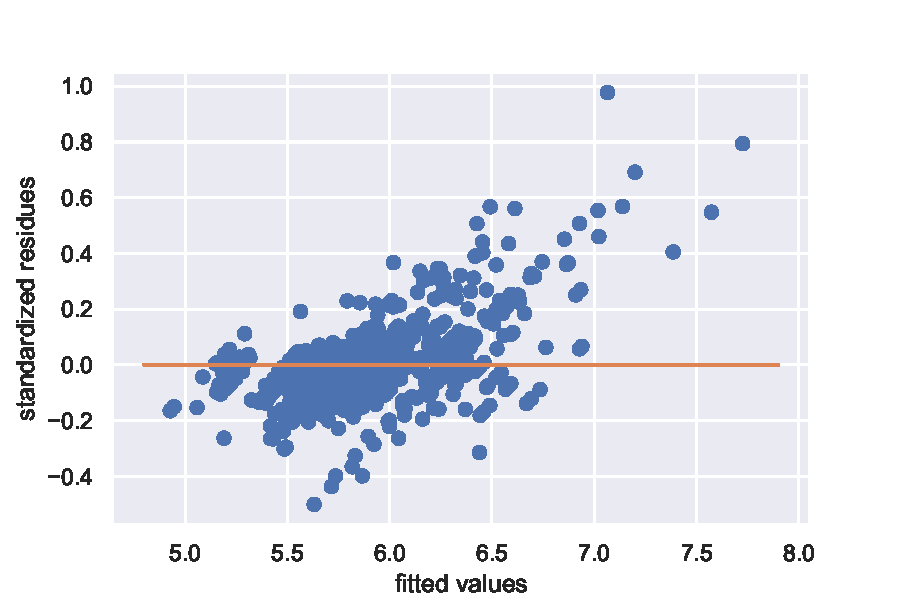
\includegraphics[width=1\linewidth]{./images/homo_mod3.pdf}
  \caption{Representation of the predicted by residual values.}
  \label{fig:homo_mod3}
\end{subfigure}%
\begin{subfigure}{.5\textwidth}
  \centering
  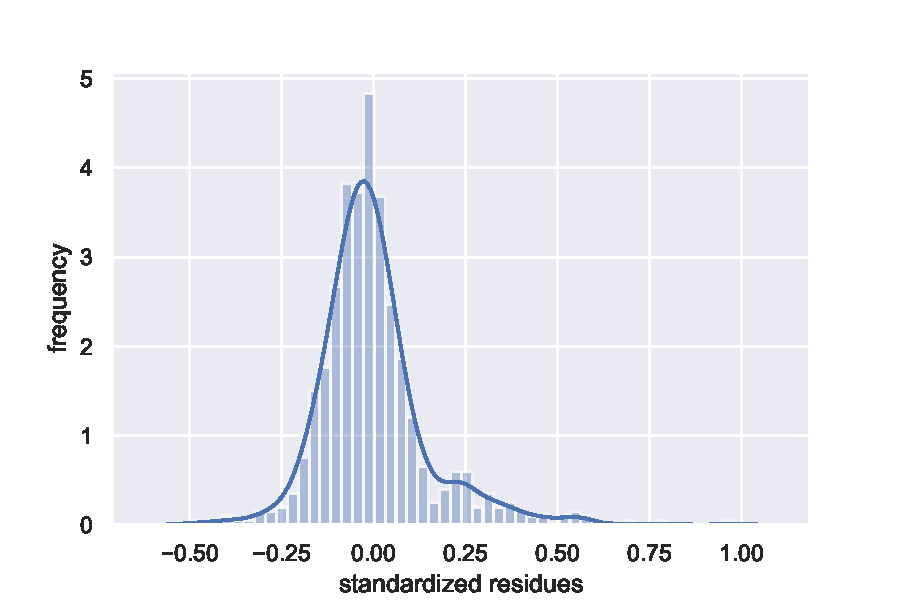
\includegraphics[width=1\linewidth, clip,trim={0cm 0cm 0cm 0.6cm} ]{./images/resid_norm_m3.pdf}
  \caption{Representation of the normality of the residuals.}
  \label{fig:resid3}
\end{subfigure}
\caption{Model validation of the third model.}
\label{fig:valid_3}
\end{figure}

In the Figure \ref{fig:valid_3}, we can see that the residues are particularly clustered around the orange line. So our model fits the data well. In addition, the normality of the residuals is also verified.

\subsection{Model selection}
We studied a total of three different models. In order to know which model is the most judicious, we compare the values of the criteria AIC and BIC.
For the model \eqref{mod3}, we obtain an AIC approximately equal to $717.1464$ (with a total of $9=8+1$ parameters) and a BIC approximately equal to $757.7387$. By comparing the AIC and BIC values of the other two models \eqref{rel:mod1} and \eqref{mod2}, we see that the model with the minimal AIC and BIC is the second \eqref{mod2}. Recall that the second model \eqref{mod2} is the model where varying intercepts and slopes, without correlation.

\begin{center}\label{summary}
    \begin{tabular}{|c|c|c|c|c|c|}
    \hline
         & parameters & deviance & loglik & $\AIC$ & $\BIC$ \\
         \hline \hline
        model 1 & 4 & 727.682 & -363.841 & 735.682 & 753.723\\
        model 2 & 5 & 699.146 & -349.573 & 709.146 & 731.598\\
        model 3 & 9 & 699.146 & -349.573 &717.146 & 757.739\\
        \hline
    \end{tabular}
    \captionof{table}{Summary of the three models.} 
\end{center}

%%%%%%%%%%%%%%%%%%%%%%%%%%%%%%%%%%%%%%%%%%%%%%%%%%%%%%%%%%%%%%%%%%%%%%%%%%%%%%%
%%%%%%%%%%%%%%%%%%%%%%%%%%%%%%%%%%%%%%%%%%%%%%%%%%%%%%%%%%%%%%%%%%%%%%%%%%%%%%%
\section*{Conclusion}
To sum up all of it, we have studied three different types of models which are
varying intercepts, varying intercepts and slopes without correlation and varying intercepts and slopes with correlation. 
For each of these, we have seen their statistical model but also how to validate it. Moreover, we used two different criteria which are AIC and BIC in order to select the least worse model for our data. Thus, in view  of their values in \ref{summary}, we can say that the least worse model is the second model \eqref{mod2} corresponding to varying intercepts and slopes without correlation.

%%%%%%%%%%%%%%%%%%%%%%%%%%%%%%%%%%%%%%%%%%%%%%%%%%%%%%%%%%%%%%%%%%%%%%%%%%%%%%%
%%%%%%%%%%%%%%%%%%%%%%%%%%%%%%%%%%%%%%%%%%%%%%%%%%%%%%%%%%%%%%%%%%%%%%%%%%%%%%%

%%%%%%%%%%%%%%%%%%%%%%%%%%%%%%%%%%%%%%%%%%%%%%%%%%%%%%%%%%%%%%%%%%%%%%%%%%%%%%%
%%%%%%%%%%%%%%%%%%%%%%%%%%%%%%%%%%%%%%%%%%%%%%%%%%%%%%%%%%%%%%%%%%%%%%%%%%%%%%%
\nocite{*}
\printbibliography
%%%%%%%%%%%%%%%%%%%%%%%%%%%%%%%%%%%%%%%%%%%%%%%%%%%%%%%%%%%%%%%%%%%%%%%%%%%%%%%
%%%%%%%%%%%%%%%%%%%%%%%%%%%%%%%%%%%%%%%%%%%%%%%%%%%%%%%%%%%%%%%%%%%%%%%%%%%%%%%

\end{document}